%!TEX TS-program = xelatex
% !TEX root = ../thesis.tex
% Do not delete; used to set build system


%\begin{savequote}[75mm] 
%Nulla facilisi. In vel sem. Morbi id urna in diam dignissim feugiat. Proin molestie tortor eu velit. Aliquam erat volutpat. Nullam ultrices, diam tempus vulputate egestas, eros pede varius leo.
%\qauthor{Quoteauthor Lastname} 
%\end{savequote}

\chapter{Supplemental algorithms and figures for ``Absolute protein quantitation: Inference with non-ignorable missing data in high throughput proteomics''}
\label{ch:supp:proteomics}

\section{Prior parameter settings}

The parameters of all priors used in our inference were selected to provide weakly-informative regularization.
Our results were generally insensitive to perturbations in these parameter values by a factor of two or more.
For $\alpha_\sigma$ and $\alpha_\tau$, the convolution parameters of our inverse-Gamma prior, we take $\log(\alpha_{\cdot}) \sim N(2.65, 1)$, which implies a prior probability of 0.95 of falling between $2$ and $100$.
This reflects a plausible range of variation while effectively ruling out degenerate cases.
For the scale parameters $\beta_\sigma$ and $\beta_\tau$, we use independent $Gamma(1, 1)$ priors.
We place uniform ($Beta(1,1)$) priors on $\pi^{rnd}$ and $\lambda$ and take $\log(r) \sim N(2.65, 1)$.

\section{Details of MCMC algorithm}
\label{supp:proteomics:sec:mcmcDetails}

\subsection{Gibbs updates for $\bm \mu$ and $\bm \gamma$}
\label{supp:proteomics:sc:draw_intensity_parameters}

Conditional on the missing data $\bm M$ and all other parameters, the conditional posterior distribution of the peptide- and protein-level mean parameters $\bm \mu$ and $\bm \gamma$ are standard Normal draws.
The conditional posterior of the peptide-level means is
\begin{equation*}h
\gamma_{ik} | \bm M, \bm \Theta_{-\gamma} \sim Normal\left(\frac{\frac{\mu_{i}}{\tau_{i}^{2}}+\frac{\bar{y}_{ik}}{\sigma_{i}^{2}/s_{ik}}}{\frac{1}{\tau_{i}^{2}}+\frac{s_{ik}}{\sigma_{i}^{2}}},\left(\frac{1}{\tau_{i}^{2}}+\frac{s_{ik}}{\sigma_{i}^{2}}\right)^{-1}\right)
\end{equation*}
Similarly, the conditional posterior distribution of the protein-level mean parameters is
\begin{equation*}
\mu_{i} | \bm M, \bm \Theta_{-\mu} \sim Normal\left(\frac{\sum_{k}\gamma_{ik}}{m_{i}},\frac{\tau_{i}^{2}}{m_{i}}\right)
\end{equation*}
. 

\subsection{Updates for variance parameters and hyperparameters}


\subsubsection{Gibbs updates for peptide- and state-level variance parameters $\bm \tau^2$ and $\bm \sigma^2$}

The peptide and state level precisions have standard conjugate conditional posterior distributions.
The conditional posterior distribution of the peptide-level precisions is 
\begin{equation*}
\frac{1}{\tau_{i}^{2}} | \bm M, \bm \Theta_{-\tau^2} \sim Gamma\left(\alpha_{\tau}+\frac{m_{i}}{2},\beta_{\tau}+\frac{1}{2}\sum_{k}(\gamma_{ik}-\mu_{i})^{2}\right) .
\end{equation*}
Similarly, the conditional posterior distribution for the state-level precisions is
\begin{equation*}
\frac{1}{\sigma_{i}^{2}} | \bm M, \bm \Theta_{-\sigma^2}  \sim Gamma\left(\alpha_{\sigma}+\frac{1}{2}\sum_{k}s_{ik},\beta_{\sigma}+\frac{1}{2}\sum_{kl}(y_{ikl}-\gamma_{ik})^{2}\right) .
\end{equation*}

\subsubsection{Metropolis-Hastings updates for variance hyperparameters}
\label{supp:proteomics:sec:var_hyperparam_updates}

As a result of our weakly-informative log-normal priors on the shape parameters $\alpha_\sigma$ and $\alpha_\tau$, their conditional posterior is not available in closed-form.
To handle these updates, we use conditional independence chain Metropolis-Hastings draws.
Throughout the below discussion, we will focus exclusively on $(\alpha_\tau, \beta_\tau)$ as the corresponding update for $(\alpha_\sigma, \beta_\sigma)$ is of identical form.

We build our proposal based on a multivariate normal approximation to the log-transformed parameters.
Specifically, we propose from a multivariate log-t distribution given by
\begin{eqnarray}
(\log \alpha_{\sigma}^*, \log \beta_{\sigma}^*) \mid \bm{\sigma} \sim \left(\begin{array}{c}
\widehat{\log\alpha_{\sigma}} \\
\widehat{\log\beta_{\sigma}}
\end{array}\right) +
\sqrt{\frac{\nu}{\nu - 2}} \hat{\mathcal{I}}(\widehat{\log\alpha_{\sigma}},\widehat{\log\beta_{\sigma}})^{-1/2} \bm{t_{\nu}} \label{supp:proteomics:eqn:alpha_and_beta_sigma_multivar_log_normal_prop}
\end{eqnarray}
where $\widehat{\log\alpha_{\sigma}}$ and $\widehat{\log\beta_{\sigma}}$ are the conditional posterior modes of $\log\alpha_{\sigma}$ and $\log\beta_\sigma$, $\hat{\mathcal{I}}(\log\alpha_\sigma,\log\beta_\sigma)$ is the negative Hessian of the log-conditional posterior evaluated at the posterior mode, and $\bm{t_{\nu}}$ is a vector of independent and identically distributed $t_{\nu}$ random variables.

To build this proposal, we must maximize $p(\log \alpha_{\sigma}, \log \beta_{\sigma} \mid \vec{\sigma})$ over $(\log \alpha_{\sigma}, \log \beta_{\sigma})$.
This requires only univariate optimization as the mode of $\log \beta_\sigma$ given $\log \alpha_\sigma$ is available in closed form:
\begin{eqnarray}
\hat{\beta}_{\sigma} = \frac{n\alpha_{\sigma} + \alpha_{0 \sigma}}{\sum_{i=1}^{n}\sigma_{i}^{-2}} .
\end{eqnarray}
We provide an example of this approximation's behavior in Figure \ref{supp:proteomics:fig:Normal-approximation-to-log-gamma-pars}.

\begin{figure}
\centering
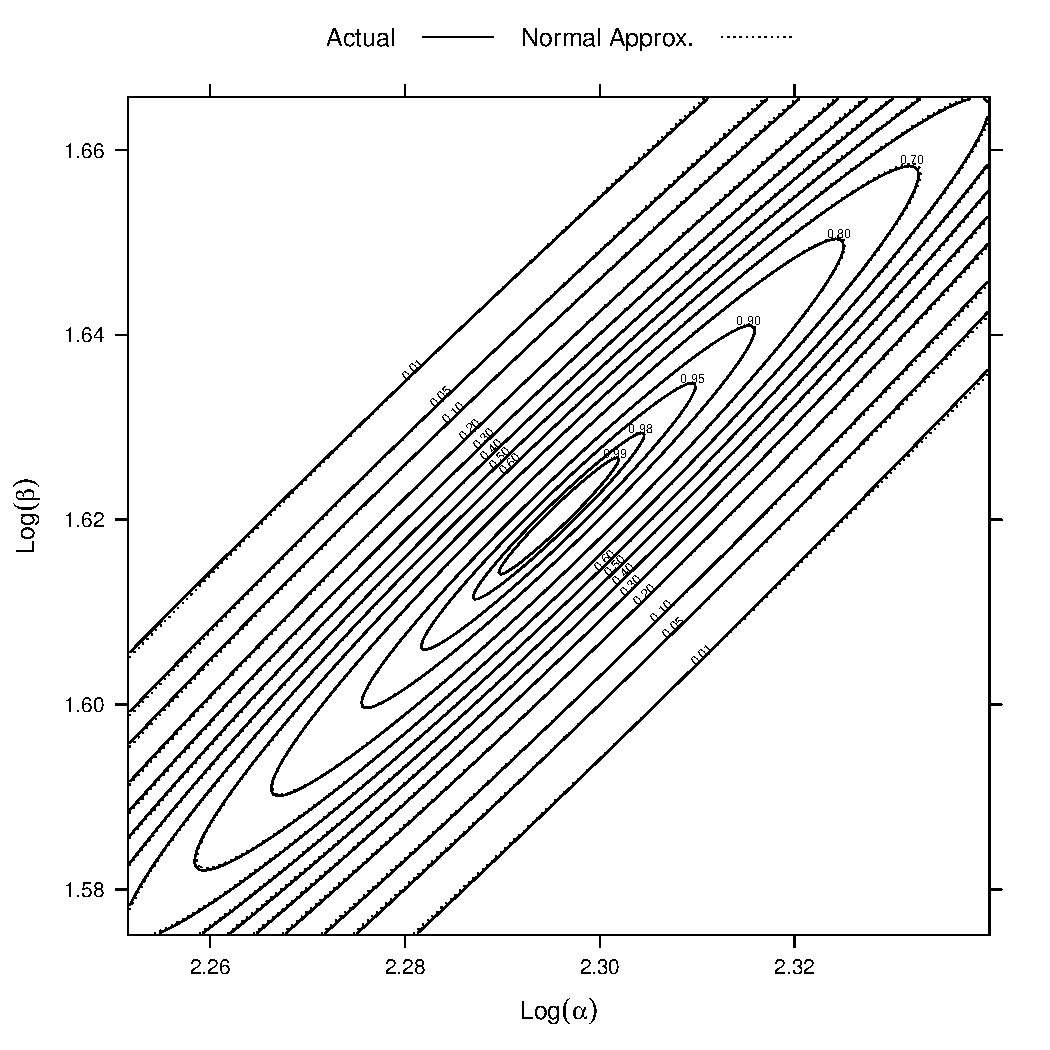
\includegraphics[width=\textwidth]{figures/proteomics/gamma_normal_approx}

\caption{Normal approximation to the conditional posterior of $(\log \alpha_\sigma, \log \beta_\sigma)$. Contours of the log-conditional posterior and proposal for $\alpha_\sigma=10$ and $\beta_\sigma=5$ with $n=1000$ observations.\label{supp:proteomics:fig:Normal-approximation-to-log-gamma-pars}} 
\end{figure}




\subsection{Updates for censoring model parameters}


\subsubsection{Gibbs update for $\pi^{rnd}$}

The conditional posterior distribution of the random censoring probability is straightforward and conjugate, enabling a direct update:
\begin{equation*}
\pi^{rnd} | \bm M, \bm \Theta_{-\pi^{rnd}} \sim Beta\left( \sum_{ikl} R_{ikl}, \sum_{ikl} (1 - R_{ikl}) \right) .
\end{equation*}


\subsubsection{Metropolis-Hastings update for intensity-based censoring parameters}

The parameters of the intensity-based censoring model, $\bm \eta$,
are updated using an independence chain Metropolis-Hastings sampler.
%
We first obtain the mode of the conditional posterior of $\bm \eta$, $\hat{\bm \eta}$, using standard GLM estimation techniques (Fisher scoring).
This estimation naturally yields the expected negative Hessian of this conditional posterior $\mathcal{I}(\hat{\bm{\eta}})$.
We then draw proposal as
\begin{equation*}
\bm{\eta}^* = \hat{\bm{\eta}} + \sqrt{\frac{\nu}{\nu - 2}} \mathcal{I}(\hat{\bm{\eta}})^{-1/2} \bm{t}_\nu,
\end{equation*}
where $\bm{t}_\nu$ is defined as before.


\subsection{Metropolis-Hastings update for number of states parameters $(r, \lambda)$}
\label{supp:proteomics:sec:draw_number_of_states_hyperparameters}

The conditional posterior distribution of $(r, \lambda)$ is not of conjugate form regardless of the prior distribution.
For our inference, we take $r \sim LogNormal(\mu_{0r}, \sigma^2_{0r})$ independent of $\lambda \sim Beta(\alpha_{0\lambda}, \beta_{0\lambda})$ a priori.
We construct a proposal for these parameters by first transforming them to $(\log r, \logit \lambda)$.
We then estimate a normal approximation to the joint conditional posterior of these transformed parameters.

As in Section \ref{supp:proteomics:sec:var_hyperparam_updates}, we can analytically maximize  the conditional posterior over one parameter given the other.
Maximizing over $\log r$ yields
%
\begin{equation*}
\widehat{\logit \lambda} = \frac{\sum_{ik}r + \alpha_{0r}}{\sum_{ik}r+\sum_{ik}(s_{ik}-1) + \alpha_{0r} + \beta_{0r}} .
\end{equation*}
%
This reduces estimation of the conditional posterior mode to univariate optimization over $\logit r$.
Following this optimization, we compute the negative Hessian of the log-conditional posteriors $\hat{\mathcal{I}}(\widehat{\log r}, \widehat{\logit \lambda})$ and propose as
\begin{equation*}
(\log r^*, \logit \lambda^*) \mid \bm s \sim \left(\begin{array}{c}
\widehat{\log r} \\
\widehat{\logit \lambda}
\end{array}\right) +
\sqrt{\frac{\nu}{\nu - 2}} \hat{\mathcal{I}}(\widehat{\log r}, \widehat{\logit \lambda})^{-1/2} \bm{t_{\nu}} .
\end{equation*}


\begin{figure}
\centering
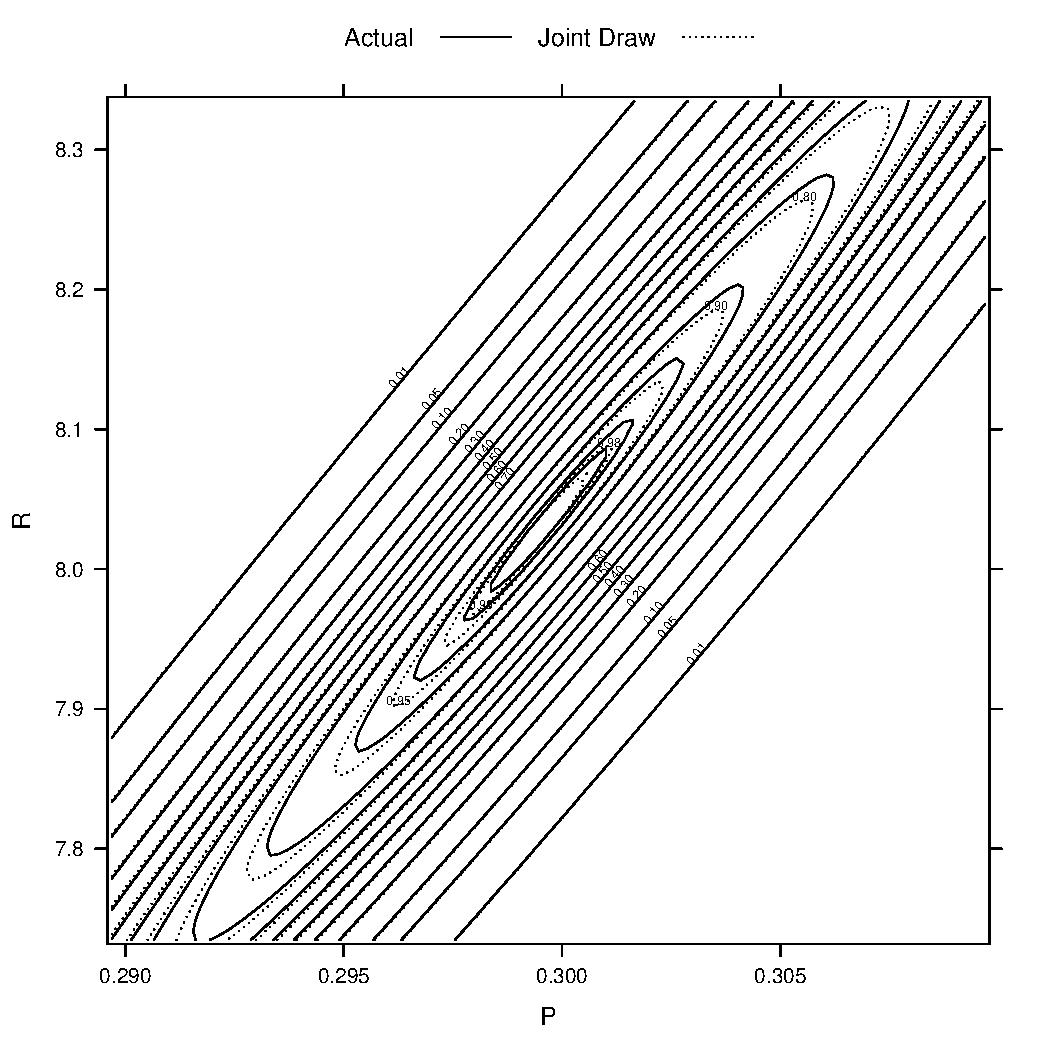
\includegraphics[width=1\textwidth]{figures/proteomics/Neg_Bin_Parameter_Draw}
\caption{Conditional posterior contours for $(r, \lambda)$.\label{supp:proteomics:fig:Negative-binomial-parameters}}
\end{figure}


 %%% %%% %%%
 %%% %%% %%%
 %%% %%% %%%

\clearpage

\section{Additional simulation results}

\begin{sidewaystable}
\begin{center}
\caption{Simulation analysis of protein abundance estimates by $\zeta_i$ and $m_i$, 90m gradient. All estimates are $\pm$ one standard deviation. \label{supp:proteomics:tab:sim_estimates_90m}}
\begin{tabular}{ccc|c|ccccc}
 Grad. & $\zeta_i$ & $m_i$ & Posterior Mean & Sum Int. & Mean Int. & Med. Int. & AMI & emPAI \\ 
  \hline
90m &   3 &  20 & $3.30 \pm 0.33$ & $2.33 \pm 0.92$ & $3.78 \pm 0.87$ & $4.85 \pm 0.77$ & $3.87 \pm 0.84$ & $5.98 \pm 0.16$ \\ 
  90m &   3 &  30 & $3.19 \pm 0.33$ & $2.38 \pm 0.78$ & $3.79 \pm 0.73$ & $4.84 \pm 0.67$ & $3.89 \pm 0.72$ & $5.84 \pm 0.19$ \\ 
  90m &   3 &  40 & $3.09 \pm 0.35$ & $2.46 \pm 0.81$ & $3.84 \pm 0.73$ & $4.89 \pm 0.64$ & $3.94 \pm 0.72$ & $5.75 \pm 0.20$ \\ 
  90m &   3 &  50 & $3.03 \pm 0.34$ & $2.40 \pm 0.76$ & $3.73 \pm 0.66$ & $4.76 \pm 0.62$ & $3.83 \pm 0.65$ & $5.68 \pm 0.21$ \\ 
  90m &   3 &  60 & $2.99 \pm 0.38$ & $2.56 \pm 0.85$ & $3.86 \pm 0.75$ & $4.86 \pm 0.64$ & $3.95 \pm 0.74$ & $5.64 \pm 0.24$ \\ 
   \hline
90m &   4 &  20 & $3.91 \pm 0.38$ & $3.23 \pm 0.68$ & $4.37 \pm 0.60$ & $5.29 \pm 0.52$ & $4.46 \pm 0.59$ & $6.32 \pm 0.24$ \\ 
  90m &   4 &  30 & $3.87 \pm 0.39$ & $3.36 \pm 0.65$ & $4.37 \pm 0.53$ & $5.22 \pm 0.45$ & $4.45 \pm 0.52$ & $6.28 \pm 0.26$ \\ 
  90m &   4 &  40 & $3.87 \pm 0.38$ & $3.57 \pm 0.64$ & $4.46 \pm 0.53$ & $5.26 \pm 0.40$ & $4.54 \pm 0.51$ & $6.27 \pm 0.26$ \\ 
  90m &   4 &  50 & $3.87 \pm 0.38$ & $3.64 \pm 0.58$ & $4.45 \pm 0.49$ & $5.26 \pm 0.37$ & $4.53 \pm 0.47$ & $6.25 \pm 0.25$ \\ 
  90m &   4 &  60 & $3.87 \pm 0.33$ & $3.76 \pm 0.55$ & $4.48 \pm 0.46$ & $5.24 \pm 0.33$ & $4.56 \pm 0.45$ & $6.26 \pm 0.22$ \\ 
   \hline
90m &   5 &  20 & $4.92 \pm 0.33$ & $4.34 \pm 0.52$ & $5.02 \pm 0.48$ & $5.67 \pm 0.29$ & $5.07 \pm 0.47$ & $6.92 \pm 0.20$ \\ 
  90m &   5 &  30 & $4.95 \pm 0.28$ & $4.61 \pm 0.49$ & $5.10 \pm 0.46$ & $5.69 \pm 0.27$ & $5.16 \pm 0.45$ & $6.93 \pm 0.16$ \\ 
  90m &   5 &  40 & $4.96 \pm 0.22$ & $4.81 \pm 0.50$ & $5.17 \pm 0.48$ & $5.68 \pm 0.23$ & $5.22 \pm 0.47$ & $6.94 \pm 0.13$ \\ 
  90m &   5 &  50 & $4.97 \pm 0.20$ & $4.89 \pm 0.44$ & $5.16 \pm 0.42$ & $5.69 \pm 0.22$ & $5.21 \pm 0.42$ & $6.94 \pm 0.12$ \\ 
  90m &   5 &  60 & $4.98 \pm 0.21$ & $4.97 \pm 0.43$ & $5.16 \pm 0.41$ & $5.66 \pm 0.19$ & $5.21 \pm 0.41$ & $6.94 \pm 0.12$ \\ 
   \hline
90m &   6 &  20 & $5.95 \pm 0.28$ & $5.48 \pm 0.50$ & $5.89 \pm 0.49$ & $6.24 \pm 0.26$ & $5.91 \pm 0.48$ & $7.36 \pm 0.14$ \\ 
  90m &   6 &  30 & $5.94 \pm 0.21$ & $5.66 \pm 0.45$ & $5.89 \pm 0.46$ & $6.23 \pm 0.23$ & $5.91 \pm 0.46$ & $7.36 \pm 0.11$ \\ 
  90m &   6 &  40 & $5.97 \pm 0.21$ & $5.83 \pm 0.45$ & $5.94 \pm 0.45$ & $6.25 \pm 0.21$ & $5.96 \pm 0.45$ & $7.36 \pm 0.10$ \\ 
  90m &   6 &  50 & $5.97 \pm 0.16$ & $5.96 \pm 0.45$ & $5.96 \pm 0.46$ & $6.25 \pm 0.18$ & $5.98 \pm 0.46$ & $7.36 \pm 0.09$ \\ 
  90m &   6 &  60 & $5.99 \pm 0.16$ & $6.04 \pm 0.42$ & $5.96 \pm 0.43$ & $6.25 \pm 0.18$ & $5.98 \pm 0.43$ & $7.37 \pm 0.08$ \\ 
   \hline
90m &   7 &  20 & $6.94 \pm 0.24$ & $6.45 \pm 0.47$ & $6.76 \pm 0.47$ & $7.03 \pm 0.25$ & $6.77 \pm 0.46$ & $7.54 \pm 0.10$ \\ 
  90m &   7 &  30 & $6.94 \pm 0.21$ & $6.65 \pm 0.43$ & $6.78 \pm 0.43$ & $7.01 \pm 0.22$ & $6.79 \pm 0.43$ & $7.56 \pm 0.09$ \\ 
  90m &   7 &  40 & $6.92 \pm 0.17$ & $6.79 \pm 0.43$ & $6.81 \pm 0.43$ & $6.99 \pm 0.19$ & $6.81 \pm 0.43$ & $7.55 \pm 0.08$ \\ 
  90m &   7 &  50 & $6.94 \pm 0.16$ & $6.96 \pm 0.46$ & $6.88 \pm 0.46$ & $7.00 \pm 0.18$ & $6.88 \pm 0.46$ & $7.55 \pm 0.07$ \\ 
  90m &   7 &  60 & $6.94 \pm 0.15$ & $7.03 \pm 0.42$ & $6.87 \pm 0.42$ & $7.01 \pm 0.16$ & $6.87 \pm 0.42$ & $7.55 \pm 0.07$ \\ 
   \hline
90m &   8 &  20 & $7.94 \pm 0.21$ & $7.46 \pm 0.45$ & $7.75 \pm 0.42$ & $7.95 \pm 0.24$ & $7.75 \pm 0.42$ & $7.59 \pm 0.09$ \\ 
  90m &   8 &  30 & $7.93 \pm 0.18$ & $7.69 \pm 0.40$ & $7.81 \pm 0.39$ & $7.93 \pm 0.21$ & $7.81 \pm 0.39$ & $7.59 \pm 0.08$ \\ 
  90m &   8 &  40 & $7.94 \pm 0.15$ & $7.83 \pm 0.40$ & $7.82 \pm 0.39$ & $7.94 \pm 0.17$ & $7.82 \pm 0.39$ & $7.60 \pm 0.07$ \\ 
  90m &   8 &  50 & $7.95 \pm 0.14$ & $7.94 \pm 0.38$ & $7.83 \pm 0.39$ & $7.96 \pm 0.17$ & $7.83 \pm 0.39$ & $7.60 \pm 0.06$ \\ 
  90m &   8 &  60 & $7.95 \pm 0.13$ & $8.01 \pm 0.34$ & $7.82 \pm 0.36$ & $7.96 \pm 0.15$ & $7.83 \pm 0.36$ & $7.60 \pm 0.06$ \\ 
   \hline
\end{tabular}
\end{center}
\end{sidewaystable}


\begin{sidewaystable}
\begin{center}
\caption{Simulation analysis of protein abundance estimates by $\zeta_i$ and $m_i$, 180m gradient. All estimates are $\pm$ one standard deviation. \label{supp:proteomics:tab:sim_estimates_180m}}
\begin{tabular}{ccc|c|ccccc}
 Grad. & $\zeta_i$ & $m_i$ & Posterior Mean & Sum Int. & Mean Int. & Med. Int. & AMI & emPAI \\ 
 \hline
180m &   3 &  20 & $3.13 \pm 0.42$ & $2.08 \pm 0.85$ & $3.46 \pm 0.80$ & $4.75 \pm 0.70$ & $3.59 \pm 0.79$ & $6.02 \pm 0.21$ \\ 
  180m &   3 &  30 & $2.97 \pm 0.44$ & $2.13 \pm 0.89$ & $3.47 \pm 0.80$ & $4.74 \pm 0.68$ & $3.60 \pm 0.79$ & $5.88 \pm 0.23$ \\ 
  180m &   3 &  40 & $2.93 \pm 0.43$ & $2.30 \pm 0.87$ & $3.56 \pm 0.76$ & $4.77 \pm 0.64$ & $3.69 \pm 0.76$ & $5.83 \pm 0.25$ \\ 
  180m &   3 &  50 & $2.91 \pm 0.44$ & $2.35 \pm 0.86$ & $3.57 \pm 0.73$ & $4.77 \pm 0.60$ & $3.69 \pm 0.72$ & $5.78 \pm 0.28$ \\ 
  180m &   3 &  60 & $2.90 \pm 0.45$ & $2.45 \pm 0.86$ & $3.59 \pm 0.72$ & $4.77 \pm 0.58$ & $3.72 \pm 0.72$ & $5.77 \pm 0.28$ \\ 
   \hline
180m &   4 &  20 & $3.89 \pm 0.47$ & $3.13 \pm 0.77$ & $4.15 \pm 0.67$ & $5.22 \pm 0.49$ & $4.26 \pm 0.66$ & $6.44 \pm 0.29$ \\ 
  180m &   4 &  30 & $3.89 \pm 0.39$ & $3.35 \pm 0.70$ & $4.20 \pm 0.62$ & $5.15 \pm 0.42$ & $4.30 \pm 0.61$ & $6.44 \pm 0.25$ \\ 
  180m &   4 &  40 & $3.91 \pm 0.36$ & $3.59 \pm 0.74$ & $4.30 \pm 0.66$ & $5.17 \pm 0.38$ & $4.41 \pm 0.65$ & $6.44 \pm 0.22$ \\ 
  180m &   4 &  50 & $3.93 \pm 0.33$ & $3.65 \pm 0.64$ & $4.26 \pm 0.57$ & $5.18 \pm 0.32$ & $4.37 \pm 0.57$ & $6.44 \pm 0.20$ \\ 
  180m &   4 &  60 & $3.93 \pm 0.33$ & $3.77 \pm 0.62$ & $4.30 \pm 0.55$ & $5.17 \pm 0.33$ & $4.41 \pm 0.54$ & $6.44 \pm 0.20$ \\ 
   \hline
180m &   5 &  20 & $4.95 \pm 0.33$ & $4.27 \pm 0.58$ & $4.87 \pm 0.55$ & $5.63 \pm 0.29$ & $4.93 \pm 0.54$ & $7.01 \pm 0.20$ \\ 
  180m &   5 &  30 & $4.97 \pm 0.28$ & $4.59 \pm 0.61$ & $5.01 \pm 0.60$ & $5.68 \pm 0.27$ & $5.07 \pm 0.59$ & $7.01 \pm 0.15$ \\ 
  180m &   5 &  40 & $4.98 \pm 0.22$ & $4.70 \pm 0.55$ & $4.98 \pm 0.55$ & $5.64 \pm 0.24$ & $5.05 \pm 0.54$ & $7.02 \pm 0.12$ \\ 
  180m &   5 &  50 & $4.99 \pm 0.19$ & $4.86 \pm 0.57$ & $5.04 \pm 0.57$ & $5.65 \pm 0.23$ & $5.11 \pm 0.57$ & $7.03 \pm 0.11$ \\ 
  180m &   5 &  60 & $5.01 \pm 0.20$ & $4.89 \pm 0.53$ & $5.00 \pm 0.53$ & $5.65 \pm 0.23$ & $5.07 \pm 0.52$ & $7.01 \pm 0.10$ \\ 
   \hline
180m &   6 &  20 & $5.96 \pm 0.28$ & $5.35 \pm 0.58$ & $5.74 \pm 0.58$ & $6.23 \pm 0.28$ & $5.77 \pm 0.57$ & $7.37 \pm 0.14$ \\ 
  180m &   6 &  30 & $5.98 \pm 0.22$ & $5.61 \pm 0.56$ & $5.81 \pm 0.57$ & $6.24 \pm 0.25$ & $5.84 \pm 0.56$ & $7.39 \pm 0.11$ \\ 
  180m &   6 &  40 & $5.96 \pm 0.18$ & $5.68 \pm 0.50$ & $5.75 \pm 0.50$ & $6.21 \pm 0.20$ & $5.78 \pm 0.50$ & $7.39 \pm 0.09$ \\ 
  180m &   6 &  50 & $5.99 \pm 0.18$ & $5.84 \pm 0.50$ & $5.82 \pm 0.50$ & $6.23 \pm 0.19$ & $5.85 \pm 0.50$ & $7.38 \pm 0.09$ \\ 
  180m &   6 &  60 & $5.99 \pm 0.16$ & $5.90 \pm 0.51$ & $5.80 \pm 0.52$ & $6.22 \pm 0.17$ & $5.83 \pm 0.52$ & $7.38 \pm 0.08$ \\ 
   \hline
180m &   7 &  20 & $6.96 \pm 0.23$ & $6.36 \pm 0.54$ & $6.68 \pm 0.55$ & $7.02 \pm 0.26$ & $6.69 \pm 0.55$ & $7.53 \pm 0.11$ \\ 
  180m &   7 &  30 & $6.94 \pm 0.21$ & $6.61 \pm 0.57$ & $6.75 \pm 0.58$ & $7.03 \pm 0.23$ & $6.76 \pm 0.58$ & $7.53 \pm 0.08$ \\ 
  180m &   7 &  40 & $6.94 \pm 0.17$ & $6.70 \pm 0.52$ & $6.71 \pm 0.54$ & $7.01 \pm 0.20$ & $6.72 \pm 0.54$ & $7.53 \pm 0.07$ \\ 
  180m &   7 &  50 & $6.94 \pm 0.16$ & $6.84 \pm 0.54$ & $6.75 \pm 0.55$ & $7.01 \pm 0.18$ & $6.75 \pm 0.55$ & $7.53 \pm 0.07$ \\ 
  180m &   7 &  60 & $6.95 \pm 0.15$ & $6.95 \pm 0.52$ & $6.78 \pm 0.54$ & $7.02 \pm 0.17$ & $6.79 \pm 0.54$ & $7.53 \pm 0.06$ \\ 
   \hline
180m &   8 &  20 & $7.91 \pm 0.21$ & $7.33 \pm 0.56$ & $7.63 \pm 0.54$ & $7.92 \pm 0.25$ & $7.63 \pm 0.54$ & $7.57 \pm 0.09$ \\ 
  180m &   8 &  30 & $7.94 \pm 0.18$ & $7.57 \pm 0.54$ & $7.69 \pm 0.53$ & $7.95 \pm 0.20$ & $7.69 \pm 0.52$ & $7.58 \pm 0.07$ \\ 
  180m &   8 &  40 & $7.94 \pm 0.14$ & $7.74 \pm 0.46$ & $7.73 \pm 0.47$ & $7.95 \pm 0.18$ & $7.73 \pm 0.47$ & $7.57 \pm 0.07$ \\ 
  180m &   8 &  50 & $7.94 \pm 0.14$ & $7.86 \pm 0.48$ & $7.76 \pm 0.50$ & $7.95 \pm 0.16$ & $7.75 \pm 0.50$ & $7.57 \pm 0.06$ \\ 
  180m &   8 &  60 & $7.94 \pm 0.13$ & $7.94 \pm 0.43$ & $7.75 \pm 0.46$ & $7.94 \pm 0.16$ & $7.75 \pm 0.46$ & $7.57 \pm 0.05$ \\ 
   \hline
\end{tabular}
\end{center}
\end{sidewaystable}


\begin{sidewaystable}
\begin{center}
\caption{Simulation analysis of protein abundance estimates by $\zeta_i$ and $m_i$, 360m gradient. All estimates are $\pm$ one standard deviation. \label{supp:proteomics:tab:sim_estimates_360m}}
\begin{tabular}{ccc|c|ccccc}
 Grad. & $\zeta_i$ & $m_i$ & Posterior Mean & Sum Int. & Mean Int. & Med. Int. & AMI & emPAI \\ 
 \hline
360m &   3 &  20 & $3.07 \pm 0.34$ & $2.25 \pm 0.67$ & $3.59 \pm 0.58$ & $4.63 \pm 0.52$ & $3.78 \pm 0.57$ & $6.02 \pm 0.24$ \\ 
  360m &   3 &  30 & $3.00 \pm 0.37$ & $2.32 \pm 0.70$ & $3.57 \pm 0.57$ & $4.57 \pm 0.44$ & $3.76 \pm 0.54$ & $5.91 \pm 0.27$ \\ 
  360m &   3 &  40 & $2.94 \pm 0.37$ & $2.45 \pm 0.67$ & $3.65 \pm 0.54$ & $4.64 \pm 0.41$ & $3.84 \pm 0.52$ & $5.84 \pm 0.28$ \\ 
  360m &   3 &  50 & $2.97 \pm 0.36$ & $2.55 \pm 0.68$ & $3.65 \pm 0.52$ & $4.61 \pm 0.41$ & $3.84 \pm 0.51$ & $5.83 \pm 0.28$ \\ 
  360m &   3 &  60 & $2.97 \pm 0.38$ & $2.65 \pm 0.67$ & $3.69 \pm 0.51$ & $4.62 \pm 0.37$ & $3.87 \pm 0.49$ & $5.83 \pm 0.30$ \\ 
   \hline
360m &   4 &  20 & $3.97 \pm 0.33$ & $3.36 \pm 0.52$ & $4.17 \pm 0.45$ & $4.95 \pm 0.30$ & $4.30 \pm 0.43$ & $6.64 \pm 0.24$ \\ 
  360m &   4 &  30 & $3.96 \pm 0.28$ & $3.59 \pm 0.47$ & $4.23 \pm 0.42$ & $4.92 \pm 0.25$ & $4.36 \pm 0.40$ & $6.63 \pm 0.20$ \\ 
  360m &   4 &  40 & $4.01 \pm 0.25$ & $3.80 \pm 0.49$ & $4.29 \pm 0.45$ & $4.95 \pm 0.23$ & $4.41 \pm 0.44$ & $6.67 \pm 0.18$ \\ 
  360m &   4 &  50 & $3.98 \pm 0.21$ & $3.85 \pm 0.45$ & $4.26 \pm 0.41$ & $4.92 \pm 0.20$ & $4.39 \pm 0.40$ & $6.64 \pm 0.15$ \\ 
  360m &   4 &  60 & $4.03 \pm 0.20$ & $3.94 \pm 0.43$ & $4.26 \pm 0.39$ & $4.92 \pm 0.21$ & $4.39 \pm 0.37$ & $6.66 \pm 0.14$ \\ 
   \hline
360m &   5 &  20 & $4.99 \pm 0.24$ & $4.46 \pm 0.42$ & $4.90 \pm 0.41$ & $5.35 \pm 0.22$ & $4.96 \pm 0.41$ & $7.21 \pm 0.15$ \\ 
  360m &   5 &  30 & $4.99 \pm 0.20$ & $4.66 \pm 0.41$ & $4.93 \pm 0.40$ & $5.36 \pm 0.20$ & $4.99 \pm 0.40$ & $7.20 \pm 0.12$ \\ 
  360m &   5 &  40 & $5.00 \pm 0.17$ & $4.85 \pm 0.41$ & $4.99 \pm 0.41$ & $5.36 \pm 0.18$ & $5.04 \pm 0.40$ & $7.21 \pm 0.10$ \\ 
  360m &   5 &  50 & $5.00 \pm 0.16$ & $4.94 \pm 0.41$ & $4.98 \pm 0.41$ & $5.35 \pm 0.16$ & $5.04 \pm 0.40$ & $7.21 \pm 0.10$ \\ 
  360m &   5 &  60 & $5.05 \pm 0.14$ & $5.05 \pm 0.39$ & $5.01 \pm 0.39$ & $5.37 \pm 0.16$ & $5.07 \pm 0.38$ & $7.21 \pm 0.08$ \\ 
   \hline
360m &   6 &  20 & $5.98 \pm 0.22$ & $5.52 \pm 0.47$ & $5.85 \pm 0.47$ & $6.07 \pm 0.24$ & $5.86 \pm 0.46$ & $7.44 \pm 0.11$ \\ 
  360m &   6 &  30 & $5.96 \pm 0.19$ & $5.71 \pm 0.44$ & $5.86 \pm 0.44$ & $6.06 \pm 0.20$ & $5.87 \pm 0.43$ & $7.43 \pm 0.10$ \\ 
  360m &   6 &  40 & $5.96 \pm 0.17$ & $5.81 \pm 0.39$ & $5.84 \pm 0.38$ & $6.06 \pm 0.16$ & $5.85 \pm 0.38$ & $7.43 \pm 0.08$ \\ 
  360m &   6 &  50 & $5.95 \pm 0.15$ & $5.94 \pm 0.40$ & $5.87 \pm 0.40$ & $6.04 \pm 0.16$ & $5.89 \pm 0.40$ & $7.43 \pm 0.07$ \\ 
  360m &   6 &  60 & $5.97 \pm 0.15$ & $6.05 \pm 0.41$ & $5.90 \pm 0.42$ & $6.05 \pm 0.16$ & $5.91 \pm 0.41$ & $7.43 \pm 0.07$ \\ 
   \hline
360m &   7 &  20 & $6.95 \pm 0.22$ & $6.52 \pm 0.44$ & $6.82 \pm 0.43$ & $6.98 \pm 0.26$ & $6.82 \pm 0.43$ & $7.48 \pm 0.10$ \\ 
  360m &   7 &  30 & $6.96 \pm 0.16$ & $6.72 \pm 0.44$ & $6.85 \pm 0.43$ & $6.99 \pm 0.19$ & $6.86 \pm 0.43$ & $7.48 \pm 0.08$ \\ 
  360m &   7 &  40 & $6.94 \pm 0.15$ & $6.85 \pm 0.38$ & $6.85 \pm 0.38$ & $6.96 \pm 0.19$ & $6.85 \pm 0.38$ & $7.48 \pm 0.07$ \\ 
  360m &   7 &  50 & $6.95 \pm 0.13$ & $6.97 \pm 0.41$ & $6.88 \pm 0.41$ & $6.97 \pm 0.16$ & $6.89 \pm 0.41$ & $7.48 \pm 0.07$ \\ 
  360m &   7 &  60 & $6.96 \pm 0.12$ & $7.06 \pm 0.41$ & $6.89 \pm 0.41$ & $6.98 \pm 0.14$ & $6.89 \pm 0.41$ & $7.48 \pm 0.06$ \\ 
   \hline
360m &   8 &  20 & $7.94 \pm 0.17$ & $7.45 \pm 0.42$ & $7.75 \pm 0.39$ & $7.96 \pm 0.21$ & $7.76 \pm 0.38$ & $7.49 \pm 0.09$ \\ 
  360m &   8 &  30 & $7.96 \pm 0.15$ & $7.71 \pm 0.38$ & $7.83 \pm 0.37$ & $7.97 \pm 0.19$ & $7.84 \pm 0.36$ & $7.48 \pm 0.08$ \\ 
  360m &   8 &  40 & $7.96 \pm 0.13$ & $7.88 \pm 0.36$ & $7.88 \pm 0.35$ & $7.96 \pm 0.16$ & $7.88 \pm 0.35$ & $7.48 \pm 0.07$ \\ 
  360m &   8 &  50 & $7.97 \pm 0.13$ & $7.96 \pm 0.34$ & $7.86 \pm 0.35$ & $7.97 \pm 0.14$ & $7.86 \pm 0.34$ & $7.49 \pm 0.06$ \\ 
  360m &   8 &  60 & $7.96 \pm 0.12$ & $8.05 \pm 0.33$ & $7.87 \pm 0.34$ & $7.97 \pm 0.14$ & $7.88 \pm 0.34$ & $7.48 \pm 0.06$ \\ 
   \hline
\end{tabular}
\end{center}
\end{sidewaystable}

% Coverage results

% latex table generated in R 2.12.2 by xtable 1.5-6 package
% Tue Apr  2 15:10:13 2013
\begin{table}
\begin{center}
\caption{Coverage of HPD posterior intervals for $\zeta_i$ in simulation study, 90m gradient
\label{supp:proteomics:tab:sim_coverage_90m}}
\begin{tabular}{ccc|cccc}
 Grad. & $\zeta_i$ & $m_i$ & 68\% & 90\% & 95\% & 99\% \\ 
  \hline
90m &   3 &  20 & 0.69 & 0.94 & 0.97 & 0.98 \\ 
  90m &   3 &  30 & 0.71 & 0.92 & 0.95 & 0.99 \\ 
  90m &   3 &  40 & 0.75 & 0.92 & 0.96 & 0.99 \\ 
  90m &   3 &  50 & 0.79 & 0.93 & 0.95 & 0.98 \\ 
  90m &   3 &  60 & 0.75 & 0.94 & 0.97 & 0.99 \\ 
   \hline
90m &   4 &  20 & 0.74 & 0.95 & 0.97 & 0.99 \\ 
  90m &   4 &  30 & 0.70 & 0.92 & 0.96 & 0.98 \\ 
  90m &   4 &  40 & 0.67 & 0.88 & 0.93 & 0.98 \\ 
  90m &   4 &  50 & 0.63 & 0.88 & 0.93 & 0.97 \\ 
  90m &   4 &  60 & 0.70 & 0.91 & 0.95 & 0.97 \\ 
   \hline
90m &   5 &  20 & 0.67 & 0.88 & 0.94 & 0.99 \\ 
  90m &   5 &  30 & 0.63 & 0.86 & 0.92 & 0.99 \\ 
  90m &   5 &  40 & 0.71 & 0.93 & 0.96 & 1.00 \\ 
  90m &   5 &  50 & 0.71 & 0.90 & 0.97 & 0.99 \\ 
  90m &   5 &  60 & 0.64 & 0.85 & 0.91 & 0.98 \\ 
   \hline
90m &   6 &  20 & 0.63 & 0.86 & 0.93 & 0.99 \\ 
  90m &   6 &  30 & 0.65 & 0.89 & 0.94 & 0.98 \\ 
  90m &   6 &  40 & 0.65 & 0.86 & 0.92 & 0.98 \\ 
  90m &   6 &  50 & 0.67 & 0.90 & 0.96 & 0.99 \\ 
  90m &   6 &  60 & 0.67 & 0.91 & 0.95 & 0.98 \\ 
   \hline
90m &   7 &  20 & 0.66 & 0.90 & 0.94 & 0.99 \\ 
  90m &   7 &  30 & 0.63 & 0.86 & 0.90 & 0.98 \\ 
  90m &   7 &  40 & 0.61 & 0.85 & 0.93 & 0.98 \\ 
  90m &   7 &  50 & 0.65 & 0.88 & 0.94 & 0.99 \\ 
  90m &   7 &  60 & 0.65 & 0.87 & 0.93 & 0.97 \\ 
   \hline
90m &   8 &  20 & 0.65 & 0.88 & 0.93 & 0.99 \\ 
  90m &   8 &  30 & 0.63 & 0.88 & 0.93 & 0.99 \\ 
  90m &   8 &  40 & 0.65 & 0.89 & 0.94 & 0.98 \\ 
  90m &   8 &  50 & 0.65 & 0.89 & 0.92 & 0.98 \\ 
  90m &   8 &  60 & 0.64 & 0.87 & 0.92 & 0.98 \\ 
   \hline
\end{tabular}
\end{center}
\end{table}

\begin{table}
\begin{center}
\caption{Coverage of HPD posterior intervals for $\zeta_i$ in simulation study, 180m gradient
\label{supp:proteomics:tab:sim_coverage_180m}}
\begin{tabular}{ccc|cccc}
 Grad. & $\zeta_i$ & $m_i$ & 68\% & 90\% & 95\% & 99\% \\ 
  \hline
180m &   3 &  20 & 0.71 & 0.91 & 0.97 & 0.99 \\ 
  180m &   3 &  30 & 0.78 & 0.91 & 0.96 & 0.99 \\ 
  180m &   3 &  40 & 0.77 & 0.93 & 0.97 & 0.99 \\ 
  180m &   3 &  50 & 0.72 & 0.92 & 0.96 & 0.99 \\ 
  180m &   3 &  60 & 0.66 & 0.90 & 0.93 & 0.98 \\ 
   \hline
180m &   4 &  20 & 0.66 & 0.89 & 0.95 & 0.99 \\ 
  180m &   4 &  30 & 0.66 & 0.89 & 0.95 & 0.98 \\ 
  180m &   4 &  40 & 0.68 & 0.88 & 0.93 & 0.97 \\ 
  180m &   4 &  50 & 0.63 & 0.87 & 0.93 & 0.97 \\ 
  180m &   4 &  60 & 0.59 & 0.86 & 0.91 & 0.97 \\ 
   \hline
180m &   5 &  20 & 0.67 & 0.87 & 0.93 & 0.97 \\ 
  180m &   5 &  30 & 0.68 & 0.90 & 0.94 & 0.98 \\ 
  180m &   5 &  40 & 0.69 & 0.90 & 0.95 & 0.99 \\ 
  180m &   5 &  50 & 0.69 & 0.90 & 0.94 & 0.99 \\ 
  180m &   5 &  60 & 0.66 & 0.87 & 0.94 & 0.98 \\ 
   \hline
180m &   6 &  20 & 0.65 & 0.88 & 0.94 & 0.98 \\ 
  180m &   6 &  30 & 0.65 & 0.92 & 0.95 & 1.00 \\ 
  180m &   6 &  40 & 0.71 & 0.88 & 0.94 & 0.99 \\ 
  180m &   6 &  50 & 0.68 & 0.86 & 0.94 & 0.98 \\ 
  180m &   6 &  60 & 0.71 & 0.89 & 0.93 & 1.00 \\ 
   \hline
180m &   7 &  20 & 0.68 & 0.91 & 0.97 & 0.99 \\ 
  180m &   7 &  30 & 0.69 & 0.88 & 0.94 & 0.97 \\ 
  180m &   7 &  40 & 0.64 & 0.87 & 0.93 & 0.98 \\ 
  180m &   7 &  50 & 0.65 & 0.87 & 0.92 & 0.97 \\ 
  180m &   7 &  60 & 0.66 & 0.88 & 0.93 & 0.98 \\ 
   \hline
180m &   8 &  20 & 0.65 & 0.88 & 0.94 & 0.99 \\ 
  180m &   8 &  30 & 0.62 & 0.87 & 0.93 & 0.98 \\ 
  180m &   8 &  40 & 0.68 & 0.90 & 0.94 & 0.98 \\ 
  180m &   8 &  50 & 0.68 & 0.87 & 0.93 & 0.97 \\ 
  180m &   8 &  60 & 0.60 & 0.86 & 0.94 & 0.98 \\ 
   \hline
\end{tabular}
\end{center}
\end{table}

\begin{table}
\begin{center}
\caption{Coverage of HPD posterior intervals for $\zeta_i$ in simulation study, 360m gradient
\label{supp:proteomics:tab:sim_coverage_360m}}
\begin{tabular}{ccc|cccc}
 Grad. & $\zeta_i$ & $m_i$ & 68\% & 90\% & 95\% & 99\% \\ 
 \hline
360m &   3 &  20 & 0.75 & 0.91 & 0.95 & 0.99 \\ 
  360m &   3 &  30 & 0.73 & 0.90 & 0.93 & 0.98 \\ 
  360m &   3 &  40 & 0.72 & 0.93 & 0.97 & 0.99 \\ 
  360m &   3 &  50 & 0.68 & 0.89 & 0.94 & 0.98 \\ 
  360m &   3 &  60 & 0.64 & 0.85 & 0.91 & 0.97 \\ 
   \hline
360m &   4 &  20 & 0.64 & 0.88 & 0.93 & 0.98 \\ 
  360m &   4 &  30 & 0.62 & 0.88 & 0.94 & 0.99 \\ 
  360m &   4 &  40 & 0.62 & 0.85 & 0.91 & 0.97 \\ 
  360m &   4 &  50 & 0.67 & 0.88 & 0.94 & 0.99 \\ 
  360m &   4 &  60 & 0.60 & 0.87 & 0.93 & 0.98 \\ 
   \hline
360m &   5 &  20 & 0.70 & 0.89 & 0.95 & 0.99 \\ 
  360m &   5 &  30 & 0.69 & 0.91 & 0.94 & 0.99 \\ 
  360m &   5 &  40 & 0.68 & 0.90 & 0.95 & 0.98 \\ 
  360m &   5 &  50 & 0.62 & 0.89 & 0.95 & 0.99 \\ 
  360m &   5 &  60 & 0.67 & 0.86 & 0.94 & 0.98 \\ 
   \hline
360m &   6 &  20 & 0.65 & 0.89 & 0.95 & 0.99 \\ 
  360m &   6 &  30 & 0.67 & 0.88 & 0.94 & 0.99 \\ 
  360m &   6 &  40 & 0.66 & 0.87 & 0.94 & 0.99 \\ 
  360m &   6 &  50 & 0.63 & 0.89 & 0.93 & 0.98 \\ 
  360m &   6 &  60 & 0.59 & 0.86 & 0.92 & 0.96 \\ 
   \hline
360m &   7 &  20 & 0.64 & 0.87 & 0.94 & 0.98 \\ 
  360m &   7 &  30 & 0.69 & 0.91 & 0.95 & 0.99 \\ 
  360m &   7 &  40 & 0.67 & 0.87 & 0.94 & 0.97 \\ 
  360m &   7 &  50 & 0.68 & 0.89 & 0.93 & 0.98 \\ 
  360m &   7 &  60 & 0.65 & 0.89 & 0.93 & 0.98 \\ 
   \hline
360m &   8 &  20 & 0.64 & 0.92 & 0.96 & 0.99 \\ 
  360m &   8 &  30 & 0.66 & 0.88 & 0.93 & 0.98 \\ 
  360m &   8 &  40 & 0.66 & 0.91 & 0.94 & 0.98 \\ 
  360m &   8 &  50 & 0.65 & 0.89 & 0.94 & 0.97 \\ 
  360m &   8 &  60 & 0.61 & 0.86 & 0.92 & 0.99 \\ 
   \hline
\end{tabular}
\end{center}
\end{table}

\begin{sidewaysfigure}
\centering
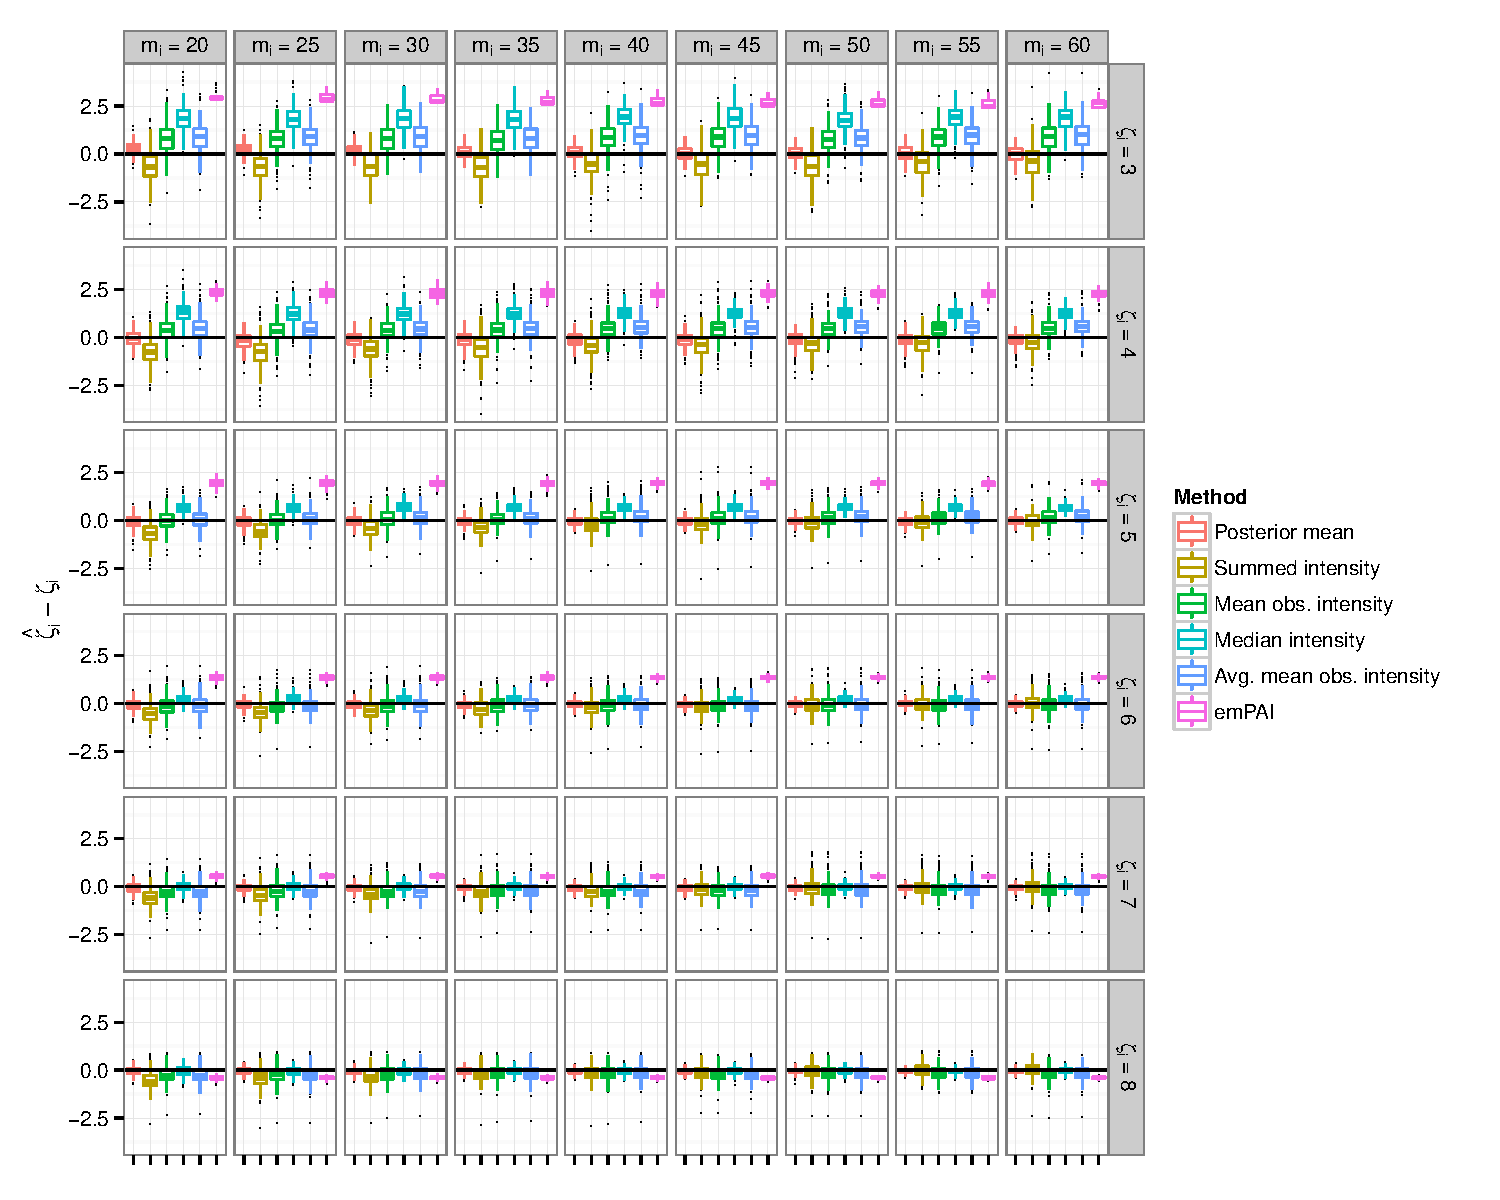
\includegraphics[height=5.25in, page=1]{figures/proteomics/figures_boxplot_sim}
\caption{Simulation results for 90m gradient.
Boxplots showing the distribution of the estimates across replicates by $m_i$ and $\zeta_i$.
Each box contains one box plot per method summarizing the fit for one combination of abundance and number of peptides.
The y-axis for all plots is $\hat{\zeta}_i - \zeta$, with a black horizontal line at zero.}
\end{sidewaysfigure}

\begin{sidewaysfigure}
\centering
\includegraphics[height=5.25in, page=2]{figures/proteomics/figures_boxplot_sim}
\caption{Simulation results for 180m gradient.
Boxplots showing the distribution of the estimates across replicates by $m_i$ and $\zeta_i$.
Each box contains one box plot per method summarizing the fit for one combination of abundance and number of peptides.
The y-axis for all plots is $\hat{\zeta}_i - \zeta$, with a black horizontal line at zero.}
\end{sidewaysfigure}

\begin{sidewaysfigure}
\centering
\includegraphics[height=5.25in, page=3]{figures/proteomics/figures_boxplot_sim}
\caption{Simulation results for 360m gradient.
Boxplots showing the distribution of the estimates across replicates by $m_i$ and $\zeta_i$.
Each box contains one box plot per method summarizing the fit for one combination of abundance and number of peptides.
The y-axis for all plots is $\hat{\zeta}_i - \zeta$, with a black horizontal line at zero.}
\end{sidewaysfigure}

 %%% %%% %%%
 %%% %%% %%%
 %%% %%% %%%

\clearpage

\section{Additional empirical results}

% latex table generated in R 2.12.2 by xtable 1.5-6 package
% Tue Apr  2 14:48:46 2013
\begin{landscape}
\begin{longtable}{cccc|cc|ccccc}
\caption{Detailed empirical results for UPS2 experiments, 90m gradients
\label{supp:proteomics:tab:ups2_90m}} \\
 Protein & $\zeta_i$ & Grad. & Rep. & $\hat{\zeta}_i$ & 90\% HPD Int. & Sum Int. & Mean Int. & Med. Int. & AMI & emPAI \\
\hline
\endfirsthead
\caption{(continued)} \\
 Protein & $\zeta_i$ & Grad. & Rep. & $\hat{\zeta}_i$ & 90\% HPD Int. & Sum Int. & Mean Int. & Med. Int. & AMI & emPAI \\
\hline
\endhead
P02788ups & -0.30 & 90m &   1 & 0.04 & $(-1.26, 1.40)$ & 1.53 & 2.58 & 2.92 & 2.71 & 2.37 \\ 
  O00762ups & 0.70 & 90m &   1 & 1.11 & $(-0.31, 2.43)$ & 1.85 & 2.90 & 3.24 & 3.03 & 2.96 \\ 
  P02787ups & 0.70 & 90m &   1 & 0.75 & $(-0.19, 1.69)$ & 2.12 & 2.87 & 3.21 & 3.00 & 2.71 \\ 
  P06396ups & 0.70 & 90m &   1 & 0.55 & $(-1.06, 2.56)$ & 3.00 & 3.75 & 3.49 & 3.58 & 2.76 \\ 
  O76070ups & 1.70 & 90m &   1 & 2.23 & $(1.29, 3.20)$ & 1.84 & 2.42 & 2.75 & 2.55 & 3.67 \\ 
  P01008ups & 1.70 & 90m &   1 & 2.03 & $(1.37, 2.61)$ & 2.36 & 2.56 & 2.77 & 2.64 & 3.54 \\ 
  P01344ups & 1.70 & 90m &   1 & 2.87 & $(1.88, 3.95)$ & 2.67 & 3.42 & 3.68 & 3.37 & 3.85 \\ 
  P08263ups & 1.70 & 90m &   1 & 2.54 & $(1.81, 3.17)$ & 2.38 & 2.65 & 2.73 & 2.78 & 3.90 \\ 
  P55957ups & 1.70 & 90m &   1 & 2.31 & $(1.42, 3.33)$ & 2.06 & 2.63 & 2.97 & 2.77 & 3.67 \\ 
  P00709ups & 2.70 & 90m &   1 & 3.00 & $(2.18, 3.86)$ & 2.53 & 2.98 & 3.22 & 3.11 & 4.00 \\ 
  P02753ups & 2.70 & 90m &   1 & 2.40 & $(1.50, 3.37)$ & 2.19 & 2.76 & 3.19 & 2.89 & 3.73 \\ 
  P06732ups & 2.70 & 90m &   1 & 2.59 & $(1.96, 3.30)$ & 3.18 & 3.33 & 3.63 & 3.46 & 3.68 \\ 
  P12081ups & 2.70 & 90m &   1 & 3.21 & $(2.67, 3.74)$ & 3.69 & 3.57 & 3.57 & 3.64 & 3.90 \\ 
  P16083ups & 2.70 & 90m &   1 & 2.55 & $(1.72, 3.39)$ & 3.02 & 3.37 & 3.26 & 3.50 & 3.73 \\ 
  P61626ups & 2.70 & 90m &   1 & 2.31 & $(1.40, 3.18)$ & 1.99 & 2.56 & 2.92 & 2.70 & 3.67 \\ 
  P63279ups & 2.70 & 90m &   1 & 2.73 & $(1.74, 3.68)$ & 2.62 & 3.19 & 2.89 & 3.33 & 3.81 \\ 
  Q15843ups & 2.70 & 90m &   1 & 1.77 & $(0.38, 3.32)$ & 1.95 & 3.00 & 3.34 & 3.14 & 3.26 \\ 
  P00167ups & 3.70 & 90m &   1 & 4.58 & $(4.03, 5.17)$ & 4.26 & 4.47 & 4.56 & 4.45 & 4.37 \\ 
  P01133ups & 3.70 & 90m &   1 & 4.08 & $(2.90, 5.34)$ & 3.25 & 4.00 & 4.34 & 4.13 & 4.23 \\ 
  P02144ups & 3.70 & 90m &   1 & 3.46 & $(2.69, 4.27)$ & 4.01 & 4.28 & 4.32 & 4.19 & 4.00 \\ 
  P04040ups & 3.70 & 90m &   1 & 4.10 & $(3.68, 4.52)$ & 4.53 & 4.23 & 4.20 & 4.28 & 4.23 \\ 
  P15559ups & 3.70 & 90m &   1 & 3.69 & $(2.87, 4.52)$ & 3.88 & 4.15 & 4.41 & 4.16 & 3.90 \\ 
  P62937ups & 3.70 & 90m &   1 & 3.17 & $(2.54, 3.81)$ & 3.52 & 3.72 & 3.16 & 3.75 & 4.00 \\ 
  P63165ups & 3.70 & 90m &   1 & 3.41 & $(2.83, 4.01)$ & 4.04 & 3.94 & 4.21 & 4.08 & 4.06 \\ 
  Q06830ups & 3.70 & 90m &   1 & 4.41 & $(3.92, 4.94)$ & 4.41 & 4.38 & 4.45 & 4.39 & 4.46 \\ 
  P00915ups & 4.70 & 90m &   1 & 4.64 & $(4.21, 5.05)$ & 4.79 & 4.69 & 4.61 & 4.67 & 4.55 \\ 
  P00918ups & 4.70 & 90m &   1 & 4.50 & $(4.05, 4.99)$ & 4.84 & 4.72 & 4.73 & 4.71 & 4.49 \\ 
  P01031ups & 4.70 & 90m &   1 & 4.21 & $(3.54, 4.87)$ & 4.26 & 4.53 & 3.95 & 4.54 & 4.62 \\ 
  P02768ups & 4.70 & 90m &   1 & 4.14 & $(3.78, 4.58)$ & 4.91 & 4.46 & 4.32 & 4.50 & 4.37 \\ 
  P41159ups & 4.70 & 90m &   1 & 3.85 & $(3.23, 4.46)$ & 4.13 & 4.28 & 3.82 & 4.27 & 4.50 \\ 
  P62988ups & 4.70 & 90m &   1 & 3.49 & $(2.79, 4.21)$ & 3.58 & 3.85 & 3.37 & 3.81 & 4.34 \\ 
  P68871ups & 4.70 & 90m &   1 & 4.62 & $(4.11, 5.20)$ & 4.67 & 4.77 & 4.66 & 4.74 & 4.42 \\ 
  P69905ups & 4.70 & 90m &   1 & 4.75 & $(4.27, 5.29)$ & 4.43 & 4.64 & 4.83 & 4.61 & 4.48 \\ 
  P02788ups & -0.30 & 90m &   2 & 0.75 & $(-0.04, 1.38)$ & 1.43 & 2.53 & 2.94 & 2.73 & 2.26 \\ 
  P01112ups & 0.70 & 90m &   2 & 2.10 & $(1.23, 2.67)$ & 1.68 & 2.48 & 2.89 & 2.68 & 3.28 \\ 
  P02787ups & 0.70 & 90m &   2 & 1.36 & $(0.78, 2.00)$ & 1.97 & 2.46 & 2.46 & 2.66 & 2.93 \\ 
  P06396ups & 0.70 & 90m &   2 & 0.74 & $(-0.05, 1.66)$ & 1.90 & 2.70 & 3.11 & 2.90 & 2.65 \\ 
  O76070ups & 1.70 & 90m &   2 & 2.69 & $(2.13, 3.27)$ & 2.16 & 2.56 & 2.69 & 2.68 & 3.90 \\ 
  P01008ups & 1.70 & 90m &   2 & 2.58 & $(2.19, 2.98)$ & 2.41 & 2.55 & 2.74 & 2.66 & 3.58 \\ 
  P01344ups & 1.70 & 90m &   2 & 3.26 & $(2.47, 4.04)$ & 2.51 & 3.30 & 3.63 & 3.33 & 3.74 \\ 
  P08263ups & 1.70 & 90m &   2 & 2.36 & $(1.87, 3.00)$ & 2.26 & 2.66 & 3.05 & 2.86 & 3.67 \\ 
  P55957ups & 1.70 & 90m &   2 & 1.07 & $(0.07, 2.43)$ & 1.70 & 2.80 & 3.21 & 3.00 & 2.98 \\ 
  P61769ups & 1.70 & 90m &   2 & 1.85 & $(0.94, 2.73)$ & 1.39 & 2.48 & 2.90 & 2.68 & 3.15 \\ 
  P00709ups & 2.70 & 90m &   2 & 3.38 & $(2.63, 3.98)$ & 2.63 & 3.12 & 3.55 & 3.33 & 3.90 \\ 
  P02753ups & 2.70 & 90m &   2 & 2.88 & $(2.07, 3.59)$ & 2.30 & 2.79 & 3.25 & 2.99 & 3.81 \\ 
  P06732ups & 2.70 & 90m &   2 & 3.24 & $(2.87, 3.60)$ & 3.38 & 3.43 & 3.69 & 3.50 & 3.78 \\ 
  P12081ups & 2.70 & 90m &   2 & 3.27 & $(2.95, 3.62)$ & 3.47 & 3.31 & 3.52 & 3.45 & 3.92 \\ 
  P16083ups & 2.70 & 90m &   2 & 3.12 & $(2.67, 3.58)$ & 3.02 & 3.22 & 3.42 & 3.36 & 3.95 \\ 
  P61626ups & 2.70 & 90m &   2 & 3.14 & $(2.75, 3.55)$ & 2.77 & 3.02 & 3.06 & 3.07 & 4.17 \\ 
  P63279ups & 2.70 & 90m &   2 & 2.77 & $(2.21, 3.59)$ & 2.53 & 3.15 & 2.77 & 3.12 & 3.70 \\ 
  Q15843ups & 2.70 & 90m &   2 & 1.84 & $(0.82, 2.91)$ & 1.86 & 2.96 & 3.37 & 3.16 & 3.15 \\ 
  P00167ups & 3.70 & 90m &   2 & 4.10 & $(3.61, 4.66)$ & 3.90 & 4.21 & 4.22 & 4.35 & 4.12 \\ 
  P01133ups & 3.70 & 90m &   2 & 3.97 & $(3.06, 5.04)$ & 3.24 & 4.04 & 4.45 & 4.24 & 4.12 \\ 
  P02144ups & 3.70 & 90m &   2 & 4.28 & $(3.91, 4.68)$ & 4.08 & 4.27 & 4.28 & 4.17 & 4.12 \\ 
  P04040ups & 3.70 & 90m &   2 & 3.91 & $(3.59, 4.30)$ & 4.46 & 4.19 & 4.10 & 4.24 & 4.16 \\ 
  P15559ups & 3.70 & 90m &   2 & 3.87 & $(3.34, 4.37)$ & 3.80 & 3.90 & 4.11 & 4.02 & 4.18 \\ 
  P62937ups & 3.70 & 90m &   2 & 3.84 & $(3.47, 4.23)$ & 3.81 & 3.90 & 3.89 & 3.93 & 4.18 \\ 
  P63165ups & 3.70 & 90m &   2 & 3.79 & $(3.44, 4.11)$ & 4.01 & 3.90 & 3.93 & 3.90 & 4.06 \\ 
  Q06830ups & 3.70 & 90m &   2 & 4.32 & $(4.03, 4.68)$ & 4.35 & 4.30 & 4.34 & 4.33 & 4.52 \\ 
  P00915ups & 4.70 & 90m &   2 & 4.74 & $(4.50, 5.03)$ & 4.77 & 4.72 & 4.74 & 4.63 & 4.44 \\ 
  P00918ups & 4.70 & 90m &   2 & 4.79 & $(4.52, 5.04)$ & 4.88 & 4.75 & 4.81 & 4.76 & 4.52 \\ 
  P01031ups & 4.70 & 90m &   2 & 4.43 & $(3.89, 5.00)$ & 4.13 & 4.52 & 4.45 & 4.65 & 4.33 \\ 
  P02768ups & 4.70 & 90m &   2 & 4.34 & $(4.07, 4.60)$ & 4.92 & 4.47 & 4.48 & 4.47 & 4.35 \\ 
  P41159ups & 4.70 & 90m &   2 & 4.37 & $(3.94, 4.86)$ & 4.47 & 4.61 & 4.57 & 4.56 & 4.52 \\ 
  P62988ups & 4.70 & 90m &   2 & 3.63 & $(3.16, 4.16)$ & 4.03 & 4.22 & 3.42 & 4.18 & 4.52 \\ 
  P68871ups & 4.70 & 90m &   2 & 4.52 & $(4.19, 4.85)$ & 4.63 & 4.73 & 4.43 & 4.65 & 4.41 \\ 
  P69905ups & 4.70 & 90m &   2 & 4.65 & $(4.33, 4.99)$ & 4.41 & 4.61 & 4.61 & 4.50 & 4.52 \\ 
   \hline
\end{longtable}
\end{landscape}
\clearpage

\begin{landscape}
\begin{longtable}{cccc|cc|ccccc}
\caption{Detailed empirical results for UPS2 experiments, 180m gradients
\label{supp:proteomics:tab:ups2_180m}} \\
 Protein & $\zeta_i$ & Grad. & Rep. & $\hat{\zeta}_i$ & 90\% HPD Int. & Sum Int. & Mean Int. & Med. Int. & AMI & emPAI \\
\hline
\endfirsthead
\caption{(continued)} \\
 Protein & $\zeta_i$ & Grad. & Rep. & $\hat{\zeta}_i$ & 90\% HPD Int. & Sum Int. & Mean Int. & Med. Int. & AMI & emPAI \\
\hline
\endhead
P02788ups & -0.30 & 180m &   1 & 0.47 & $(-0.48, 1.40)$ & 0.68 & 1.76 & 2.14 & 1.91 & 2.39 \\ 
  O00762ups & 0.70 & 180m &   1 & 1.36 & $(0.48, 2.27)$ & 1.61 & 2.69 & 2.77 & 2.54 & 2.98 \\ 
  P02787ups & 0.70 & 180m &   1 & 0.72 & $(-0.41, 1.74)$ & 3.12 & 3.73 & 3.24 & 3.88 & 2.92 \\ 
  P06396ups & 0.70 & 180m &   1 & 1.05 & $(0.05, 2.15)$ & 3.06 & 3.67 & 3.18 & 3.60 & 2.96 \\ 
  O76070ups & 1.70 & 180m &   1 & 2.73 & $(2.12, 3.36)$ & 2.30 & 2.69 & 2.89 & 2.76 & 4.02 \\ 
  P01008ups & 1.70 & 180m &   1 & 1.45 & $(0.60, 2.45)$ & 1.90 & 2.51 & 2.76 & 2.54 & 3.12 \\ 
  P01344ups & 1.70 & 180m &   1 & 3.36 & $(2.52, 4.19)$ & 2.62 & 3.22 & 3.49 & 3.25 & 4.16 \\ 
  P08263ups & 1.70 & 180m &   1 & 1.65 & $(0.80, 2.47)$ & 1.71 & 2.49 & 2.87 & 2.64 & 3.28 \\ 
  P55957ups & 1.70 & 180m &   1 & 2.34 & $(1.44, 3.21)$ & 2.62 & 3.23 & 3.31 & 3.16 & 3.69 \\ 
  P00709ups & 2.70 & 180m &   1 & 2.35 & $(1.39, 3.31)$ & 2.22 & 3.00 & 3.26 & 2.98 & 3.58 \\ 
  P02753ups & 2.70 & 180m &   1 & 2.81 & $(1.92, 3.89)$ & 2.93 & 3.53 & 3.31 & 3.69 & 3.75 \\ 
  P06732ups & 2.70 & 180m &   1 & 2.63 & $(1.94, 3.24)$ & 3.19 & 3.31 & 3.33 & 3.42 & 3.78 \\ 
  P12081ups & 2.70 & 180m &   1 & 3.02 & $(2.66, 3.41)$ & 3.31 & 3.14 & 3.21 & 3.21 & 4.05 \\ 
  P16083ups & 2.70 & 180m &   1 & 2.84 & $(2.27, 3.39)$ & 2.79 & 3.10 & 3.11 & 3.13 & 3.87 \\ 
  P61626ups & 2.70 & 180m &   1 & 2.46 & $(1.76, 3.14)$ & 2.19 & 2.67 & 2.99 & 2.73 & 3.87 \\ 
  P63279ups & 2.70 & 180m &   1 & 2.54 & $(1.22, 3.80)$ & 2.41 & 3.19 & 3.57 & 3.35 & 3.58 \\ 
  Q15843ups & 2.70 & 180m &   1 & 2.34 & $(1.23, 3.54)$ & 2.01 & 2.79 & 3.17 & 2.94 & 3.66 \\ 
  P00167ups & 3.70 & 180m &   1 & 3.78 & $(2.76, 4.85)$ & 3.68 & 4.16 & 4.52 & 4.31 & 3.94 \\ 
  P01133ups & 3.70 & 180m &   1 & 4.28 & $(3.27, 5.50)$ & 3.57 & 4.35 & 4.73 & 4.50 & 4.25 \\ 
  P02144ups & 3.70 & 180m &   1 & 3.88 & $(2.94, 4.81)$ & 3.70 & 4.09 & 4.24 & 4.16 & 3.90 \\ 
  P04040ups & 3.70 & 180m &   1 & 3.92 & $(3.58, 4.29)$ & 4.40 & 4.08 & 3.89 & 4.09 & 4.36 \\ 
  P15559ups & 3.70 & 180m &   1 & 3.53 & $(2.87, 4.17)$ & 3.84 & 4.07 & 3.77 & 4.03 & 4.02 \\ 
  P62937ups & 3.70 & 180m &   1 & 3.54 & $(2.92, 4.16)$ & 3.72 & 3.90 & 3.90 & 3.92 & 4.13 \\ 
  P63165ups & 3.70 & 180m &   1 & 3.34 & $(2.95, 3.72)$ & 3.73 & 3.58 & 3.41 & 3.60 & 4.23 \\ 
  Q06830ups & 3.70 & 180m &   1 & 4.11 & $(3.59, 4.65)$ & 3.98 & 4.06 & 4.09 & 4.13 & 4.31 \\ 
  P00915ups & 4.70 & 180m &   1 & 5.07 & $(4.81, 5.37)$ & 4.90 & 4.90 & 5.00 & 4.84 & 4.41 \\ 
  P00918ups & 4.70 & 180m &   1 & 4.59 & $(4.19, 5.05)$ & 4.76 & 4.69 & 4.79 & 4.72 & 4.44 \\ 
  P01031ups & 4.70 & 180m &   1 & 3.71 & $(3.01, 4.40)$ & 3.90 & 4.21 & 4.02 & 4.24 & 4.64 \\ 
  P02768ups & 4.70 & 180m &   1 & 4.50 & $(4.21, 4.80)$ & 5.17 & 4.72 & 4.49 & 4.69 & 4.45 \\ 
  P41159ups & 4.70 & 180m &   1 & 3.67 & $(3.02, 4.34)$ & 4.18 & 4.42 & 3.64 & 4.42 & 4.39 \\ 
  P62988ups & 4.70 & 180m &   1 & 3.96 & $(3.39, 4.56)$ & 4.16 & 4.47 & 4.14 & 4.36 & 4.35 \\ 
  P68871ups & 4.70 & 180m &   1 & 4.22 & $(3.70, 4.77)$ & 4.42 & 4.50 & 4.44 & 4.51 & 4.54 \\ 
  P69905ups & 4.70 & 180m &   1 & 4.62 & $(4.18, 5.05)$ & 4.32 & 4.56 & 4.44 & 4.44 & 4.50 \\ 
  P02788ups & -0.30 & 180m &   2 & 0.22 & $(-0.55, 1.03)$ & 0.97 & 2.04 & 2.51 & 2.29 & 2.22 \\ 
  P01112ups & 0.70 & 180m &   2 & 1.51 & $(0.77, 2.27)$ & 1.75 & 2.52 & 2.99 & 2.77 & 3.23 \\ 
  P02787ups & 0.70 & 180m &   2 & 1.06 & $(0.57, 1.56)$ & 1.72 & 2.19 & 2.14 & 2.34 & 2.88 \\ 
  P06396ups & 0.70 & 180m &   2 & 1.14 & $(0.63, 1.64)$ & 2.10 & 2.47 & 2.37 & 2.64 & 3.04 \\ 
  P51965ups & 0.70 & 180m &   2 & 0.72 & $(-0.16, 1.56)$ & 0.24 & 1.31 & 1.78 & 1.56 & 2.93 \\ 
  P99999ups & 0.70 & 180m &   2 & 2.15 & $(0.93, 3.31)$ & 1.76 & 2.83 & 3.00 & 2.78 & 3.11 \\ 
  O76070ups & 1.70 & 180m &   2 & 2.20 & $(1.64, 2.71)$ & 1.81 & 2.10 & 2.69 & 2.35 & 3.99 \\ 
  P01008ups & 1.70 & 180m &   2 & 1.88 & $(1.48, 2.31)$ & 2.22 & 2.39 & 2.39 & 2.54 & 3.46 \\ 
  P01344ups & 1.70 & 180m &   2 & 2.93 & $(2.43, 3.47)$ & 2.45 & 2.82 & 2.83 & 2.93 & 4.47 \\ 
  P08263ups & 1.70 & 180m &   2 & 2.48 & $(1.95, 2.97)$ & 2.74 & 2.96 & 2.69 & 3.06 & 3.85 \\ 
  P10599ups & 1.70 & 180m &   2 & 1.94 & $(1.04, 2.84)$ & 1.43 & 2.20 & 2.67 & 2.45 & 3.41 \\ 
  P55957ups & 1.70 & 180m &   2 & 2.64 & $(2.08, 3.21)$ & 2.52 & 2.81 & 3.21 & 2.99 & 3.99 \\ 
  P61769ups & 1.70 & 180m &   2 & 1.91 & $(0.44, 3.67)$ & 2.04 & 3.11 & 3.57 & 3.35 & 3.11 \\ 
  P00709ups & 2.70 & 180m &   2 & 3.06 & $(2.49, 3.63)$ & 2.85 & 3.22 & 3.14 & 3.26 & 4.02 \\ 
  P02753ups & 2.70 & 180m &   2 & 2.93 & $(2.42, 3.48)$ & 2.55 & 2.85 & 3.05 & 3.03 & 4.08 \\ 
  P06732ups & 2.70 & 180m &   2 & 3.20 & $(2.87, 3.56)$ & 3.31 & 3.23 & 3.24 & 3.28 & 3.90 \\ 
  P12081ups & 2.70 & 180m &   2 & 3.26 & $(2.98, 3.56)$ & 3.59 & 3.33 & 3.15 & 3.41 & 3.99 \\ 
  P16083ups & 2.70 & 180m &   2 & 3.09 & $(2.75, 3.44)$ & 3.01 & 3.00 & 3.29 & 3.15 & 4.24 \\ 
  P61626ups & 2.70 & 180m &   2 & 3.38 & $(2.94, 3.86)$ & 3.09 & 3.31 & 3.46 & 3.45 & 4.12 \\ 
  P63279ups & 2.70 & 180m &   2 & 2.96 & $(2.32, 3.58)$ & 2.65 & 3.12 & 3.39 & 3.19 & 3.85 \\ 
  Q15843ups & 2.70 & 180m &   2 & 2.64 & $(2.07, 3.20)$ & 2.31 & 2.78 & 2.81 & 2.78 & 3.95 \\ 
  P00167ups & 3.70 & 180m &   2 & 4.49 & $(4.06, 4.96)$ & 4.14 & 4.37 & 4.41 & 4.51 & 4.21 \\ 
  P01133ups & 3.70 & 180m &   2 & 3.34 & $(2.66, 4.07)$ & 2.62 & 3.39 & 3.38 & 3.24 & 4.08 \\ 
  P02144ups & 3.70 & 180m &   2 & 4.36 & $(4.04, 4.69)$ & 4.11 & 4.23 & 4.36 & 4.28 & 4.18 \\ 
  P04040ups & 3.70 & 180m &   2 & 4.04 & $(3.79, 4.27)$ & 4.49 & 4.16 & 4.05 & 4.14 & 4.19 \\ 
  P15559ups & 3.70 & 180m &   2 & 4.07 & $(3.74, 4.42)$ & 4.01 & 4.04 & 4.03 & 4.12 & 4.22 \\ 
  P62937ups & 3.70 & 180m &   2 & 3.83 & $(3.46, 4.17)$ & 3.96 & 3.95 & 4.18 & 3.98 & 4.31 \\ 
  P63165ups & 3.70 & 180m &   2 & 3.60 & $(3.34, 3.87)$ & 4.14 & 3.87 & 3.64 & 3.87 & 4.29 \\ 
  Q06830ups & 3.70 & 180m &   2 & 4.32 & $(3.99, 4.65)$ & 4.24 & 4.26 & 4.42 & 4.32 & 4.22 \\ 
  P00915ups & 4.70 & 180m &   2 & 4.73 & $(4.46, 4.99)$ & 4.85 & 4.78 & 4.88 & 4.79 & 4.39 \\ 
  P00918ups & 4.70 & 180m &   2 & 4.76 & $(4.47, 5.04)$ & 4.80 & 4.76 & 4.86 & 4.78 & 4.20 \\ 
  P01031ups & 4.70 & 180m &   2 & 4.19 & $(3.67, 4.71)$ & 3.82 & 4.11 & 4.10 & 4.29 & 4.47 \\ 
  P02768ups & 4.70 & 180m &   2 & 4.41 & $(4.20, 4.63)$ & 4.90 & 4.43 & 4.50 & 4.48 & 4.30 \\ 
  P41159ups & 4.70 & 180m &   2 & 4.52 & $(4.17, 4.88)$ & 4.39 & 4.61 & 4.32 & 4.56 & 4.21 \\ 
  P62988ups & 4.70 & 180m &   2 & 4.08 & $(3.68, 4.49)$ & 3.85 & 4.14 & 4.14 & 4.09 & 4.18 \\ 
  P68871ups & 4.70 & 180m &   2 & 4.44 & $(4.04, 4.81)$ & 4.53 & 4.70 & 4.48 & 4.62 & 4.15 \\ 
  P69905ups & 4.70 & 180m &   2 & 4.66 & $(4.33, 5.00)$ & 4.57 & 4.80 & 4.64 & 4.63 & 4.33 \\ 
   \hline
\end{longtable}
\end{landscape}
\clearpage


\begin{landscape}
\begin{longtable}{cccc|cc|ccccc}
\caption{Detailed empirical results for UPS2 experiments, 360m gradient
\label{supp:proteomics:tab:ups2_360m}} \\
 Protein & $\zeta_i$ & Grad. & Rep. & $\hat{\zeta}_i$ & 90\% HPD Int. & Sum Int. & Mean Int. & Med. Int. & AMI & emPAI \\
\hline
\endfirsthead
\caption{(continued)} \\
 Protein & $\zeta_i$ & Grad. & Rep. & $\hat{\zeta}_i$ & 90\% HPD Int. & Sum Int. & Mean Int. & Med. Int. & AMI & emPAI \\
\hline
\endhead
P02788ups & -0.30 & 360m &   1 & 0.49 & $(-0.17, 1.21)$ & 1.17 & 1.78 & 2.17 & 2.03 & 2.69 \\ 
  O00762ups & 0.70 & 360m &   1 & 1.19 & $(0.46, 1.84)$ & 1.03 & 1.64 & 2.32 & 1.89 & 3.34 \\ 
  P01112ups & 0.70 & 360m &   1 & 1.76 & $(1.08, 2.49)$ & 1.71 & 2.32 & 2.66 & 2.45 & 3.43 \\ 
  P02787ups & 0.70 & 360m &   1 & 0.80 & $(0.10, 1.48)$ & 2.00 & 2.48 & 2.43 & 2.74 & 2.86 \\ 
  P06396ups & 0.70 & 360m &   1 & 1.02 & $(0.46, 1.62)$ & 2.00 & 2.40 & 2.54 & 2.57 & 3.01 \\ 
  P09211ups & 0.70 & 360m &   1 & 0.80 & $(-0.14, 1.79)$ & 0.66 & 1.75 & 2.30 & 2.01 & 2.82 \\ 
  P99999ups & 0.70 & 360m &   1 & 1.21 & $(0.16, 2.22)$ & 0.79 & 1.88 & 2.43 & 2.13 & 3.08 \\ 
  O76070ups & 1.70 & 360m &   1 & 2.47 & $(1.98, 2.96)$ & 2.30 & 2.61 & 2.64 & 2.69 & 3.97 \\ 
  P01008ups & 1.70 & 360m &   1 & 2.15 & $(1.72, 2.57)$ & 2.40 & 2.45 & 2.53 & 2.60 & 3.64 \\ 
  P01344ups & 1.70 & 360m &   1 & 3.12 & $(2.46, 3.73)$ & 2.30 & 2.79 & 3.16 & 2.95 & 4.22 \\ 
  P08263ups & 1.70 & 360m &   1 & 2.60 & $(2.13, 3.06)$ & 2.48 & 2.67 & 2.85 & 2.78 & 3.93 \\ 
  P10599ups & 1.70 & 360m &   1 & 1.95 & $(0.96, 3.05)$ & 1.49 & 2.28 & 2.83 & 2.53 & 3.38 \\ 
  P55957ups & 1.70 & 360m &   1 & 2.66 & $(2.16, 3.14)$ & 2.39 & 2.64 & 2.88 & 2.78 & 4.09 \\ 
  P61769ups & 1.70 & 360m &   1 & 2.50 & $(1.53, 3.37)$ & 2.01 & 2.62 & 3.03 & 2.87 & 3.72 \\ 
  P00709ups & 2.70 & 360m &   1 & 2.68 & $(1.97, 3.39)$ & 2.53 & 2.92 & 3.33 & 3.09 & 4.00 \\ 
  P02753ups & 2.70 & 360m &   1 & 3.17 & $(2.61, 3.74)$ & 2.50 & 2.82 & 3.23 & 3.07 & 4.05 \\ 
  P06732ups & 2.70 & 360m &   1 & 3.32 & $(3.03, 3.61)$ & 3.39 & 3.27 & 3.32 & 3.30 & 3.99 \\ 
  P12081ups & 2.70 & 360m &   1 & 2.94 & $(2.66, 3.21)$ & 3.36 & 3.04 & 2.98 & 3.15 & 4.15 \\ 
  P16083ups & 2.70 & 360m &   1 & 3.11 & $(2.71, 3.49)$ & 3.09 & 3.13 & 3.25 & 3.25 & 4.14 \\ 
  P61626ups & 2.70 & 360m &   1 & 3.09 & $(2.45, 3.80)$ & 2.63 & 3.03 & 3.28 & 3.20 & 3.83 \\ 
  P63279ups & 2.70 & 360m &   1 & 2.59 & $(1.96, 3.23)$ & 2.30 & 2.91 & 2.74 & 2.86 & 3.63 \\ 
  Q15843ups & 2.70 & 360m &   1 & 2.50 & $(1.65, 3.38)$ & 2.27 & 3.06 & 3.30 & 3.02 & 3.46 \\ 
  P00167ups & 3.70 & 360m &   1 & 4.67 & $(4.26, 5.08)$ & 4.02 & 4.34 & 4.66 & 4.46 & 4.05 \\ 
  P01133ups & 3.70 & 360m &   1 & 3.65 & $(2.96, 4.32)$ & 2.99 & 3.78 & 3.55 & 3.56 & 4.05 \\ 
  P02144ups & 3.70 & 360m &   1 & 4.20 & $(3.83, 4.59)$ & 4.34 & 4.47 & 4.24 & 4.45 & 4.16 \\ 
  P04040ups & 3.70 & 360m &   1 & 3.94 & $(3.72, 4.18)$ & 4.39 & 4.07 & 4.00 & 4.03 & 4.20 \\ 
  P15559ups & 3.70 & 360m &   1 & 4.01 & $(3.72, 4.34)$ & 3.97 & 4.02 & 3.86 & 4.02 & 4.20 \\ 
  P62937ups & 3.70 & 360m &   1 & 3.84 & $(3.49, 4.25)$ & 3.88 & 3.93 & 4.05 & 3.95 & 4.20 \\ 
  P63165ups & 3.70 & 360m &   1 & 3.69 & $(3.41, 3.98)$ & 4.20 & 3.94 & 3.76 & 3.94 & 4.27 \\ 
  Q06830ups & 3.70 & 360m &   1 & 4.61 & $(4.35, 4.88)$ & 4.35 & 4.33 & 4.52 & 4.47 & 4.37 \\ 
  P00915ups & 4.70 & 360m &   1 & 4.81 & $(4.55, 5.06)$ & 4.77 & 4.78 & 4.77 & 4.73 & 4.22 \\ 
  P00918ups & 4.70 & 360m &   1 & 4.51 & $(4.17, 4.83)$ & 4.82 & 4.68 & 4.75 & 4.74 & 4.45 \\ 
  P01031ups & 4.70 & 360m &   1 & 4.21 & $(3.71, 4.73)$ & 3.90 & 4.22 & 4.19 & 4.34 & 4.45 \\ 
  P02768ups & 4.70 & 360m &   1 & 4.31 & $(4.09, 4.53)$ & 4.93 & 4.46 & 4.47 & 4.47 & 4.31 \\ 
  P41159ups & 4.70 & 360m &   1 & 4.48 & $(4.10, 4.88)$ & 4.56 & 4.70 & 4.45 & 4.65 & 4.45 \\ 
  P62988ups & 4.70 & 360m &   1 & 3.99 & $(3.59, 4.39)$ & 4.03 & 4.27 & 4.01 & 4.17 & 4.30 \\ 
  P68871ups & 4.70 & 360m &   1 & 4.45 & $(4.03, 4.89)$ & 4.42 & 4.56 & 4.60 & 4.62 & 4.24 \\ 
  P69905ups & 4.70 & 360m &   1 & 4.61 & $(4.29, 4.95)$ & 4.50 & 4.75 & 4.70 & 4.57 & 4.30 \\ 
   \hline
\end{longtable}
\end{landscape}
\clearpage
